\documentclass[11pt,a4paper]{article}
\usepackage[margin=0.82in,headheight=15pt,headsep=18pt]{geometry}
\usepackage[T1]{fontenc}
\usepackage{mathptmx}
\usepackage[scaled=0.94]{helvet}
\usepackage{microtype,graphicx,tikz,pgfplots,booktabs,array,tabularx}
\usepackage{xcolor,caption,fancyhdr,titlesec,hyperref}
\usetikzlibrary{arrows.meta,positioning,calc}
\pgfplotsset{compat=1.18}
\definecolor{ink}{HTML}{192C3B}
\definecolor{accent}{HTML}{23685E}
\definecolor{muted}{HTML}{56636C}
\definecolor{chipgray}{HTML}{F0F1F2}
\definecolor{linegray}{HTML}{D8DEE1}
\hypersetup{colorlinks=true,linkcolor=accent,urlcolor=accent,pdftitle={Hypothesis-Tree Agents for Molecular Discovery},pdfauthor={}}
\setlength{\parindent}{0pt}
\setlength{\parskip}{7pt}
\linespread{1.07}
\titleformat{\section}{\Large\sffamily\bfseries\color{ink}}{\thesection.}{0.5em}{}
\titlespacing*{\section}{0pt}{14pt}{9pt}
\titleformat{\subsection}{\normalsize\sffamily\bfseries\color{accent}}{}{0pt}{}
\titlespacing*{\subsection}{0pt}{11pt}{3pt}
\captionsetup{hypcap=false,font=small,labelfont=bf,justification=raggedright,singlelinecheck=false,skip=7pt}
\pagestyle{fancy}\fancyhf{}
\fancyhead[L]{\footnotesize\sffamily\color{muted}HYPOTHESIS-TREE AGENTS}
\fancyhead[R]{\footnotesize\sffamily\color{muted}RESEARCH PROPOSAL}
\fancyfoot[L]{\footnotesize\sffamily\color{muted}October 2026}
\fancyfoot[R]{\footnotesize\sffamily\color{muted}\thepage}
\renewcommand{\headrulewidth}{0.3pt}
\newcommand{\chip}[1]{\tikz[baseline=(label.base)]\node[fill=chipgray,rounded corners=2pt,inner xsep=5pt,inner ysep=3pt,font=\normalfont\normalsize] (label) {\strut #1};}
\newcommand{\level}[1]{\subsection*{#1}}
\tikzset{flow/.style={draw=linegray,fill=chipgray,rounded corners=4pt,align=left,inner sep=9pt,font=\small,text width=4.65cm,minimum height=1.3cm}, arrow/.style={-{Latex[length=2mm]},line width=.8pt,draw=accent}}
\begin{document}
\thispagestyle{fancy}
{\small\sffamily\bfseries\color{accent}AUTONOMOUS SCIENTIFIC DISCOVERY}\par\vspace{7pt}
{\fontsize{27}{30}\selectfont\sffamily\bfseries\color{ink}Hypothesis-Tree Agents\\for Molecular Discovery}\par
\vspace{4pt}
{\large\color{muted}Learning from experiments through persistent scientific memory}\par
\vspace{12pt}
\colorbox{chipgray}{\parbox{\dimexpr\linewidth-2\fboxsep\relax}{\vspace{6pt}\textbf{Proposal in brief.} Build a molecular research agent that turns each experiment into a reusable paper, selects its next question from a branching research history, and improves a hidden objective through evidence-guided experimentation.\vspace{6pt}}}

\section{Introduction}
Molecular discovery is a sequential learning problem: each candidate should teach us something useful about the next experiment. A black-box oracle makes this particularly demanding. The agent can submit a molecular structure and observe a scalar score, but cannot inspect the objective's formula or gradients. The central research question is whether an agent can make these evaluations more informative by maintaining an explicit record of what it tried, what improved, what failed, and which explanations remain uncertain.

We propose a \textbf{hypothesis tree} as the agent's scientific memory. Each node represents a testable hypothesis and its completed experiment, documented as a short research paper. A child builds on a committed parent; siblings test distinct claims arising from the same research state. This organization lets the agent deepen a promising lineage, revisit an earlier question, or compare evidence across branches without discarding negative results. The tree therefore stores both successful molecules and the reasoning needed to design subsequent tests.

A Qwen language model operates through a ReAct loop: it reasons about the current evidence, chooses a structured action, observes the result, and revises its next step. Persistent notes support work in progress; published papers preserve the verified experimental record. The intended contribution is an agent that improves its \emph{experimental decisions} as evidence accumulates, without requiring model-weight updates during a campaign.

\begin{center}
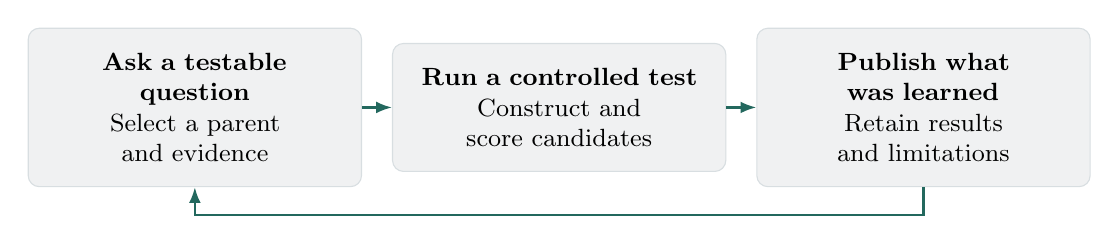
\begin{tikzpicture}[font=\small,every node/.style={align=center}]
\node[flow,text width=3.6cm,align=center] (q) {\textbf{Ask a testable question}\\Select a parent and evidence};
\node[flow,text width=3.6cm,align=center,right=0.38cm of q] (e) {\textbf{Run a controlled test}\\Construct and score candidates};
\node[flow,text width=3.6cm,align=center,right=0.38cm of e] (p) {\textbf{Publish what was learned}\\Retain results and limitations};
\draw[arrow] (q)--(e);\draw[arrow](e)--(p);
\draw[arrow] (p.south)--++(0,-.35)-|(q.south);
\end{tikzpicture}
\end{center}
The campaign examined here improved the measured score from \textbf{0.368 to 0.905}, with \textbf{83 unique scored molecules including initialization} and \textbf{48 completed experiment papers}. These results motivate a broader evaluation of whether structured scientific memory improves discovery efficiency and the quality of the hypotheses an agent chooses.

\newpage
\section{Action space}
The action interface makes scientific work explicit. Each turn returns a structured envelope, \textsf{\{reason, action, args\}}, containing a concise rationale and one action. The available actions depend on the current phase, while reads and notes can recur as often as needed within that phase.

\renewcommand{\arraystretch}{1.2}
\begin{tabularx}{\linewidth}{@{}p{0.40\linewidth}X@{}}
\toprule
\textbf{Action} & \textbf{Scientific purpose}\\
\midrule
\chip{inspect\_tree} & View paginated node summaries and locate promising or unresolved research lines.\\[7pt]
\chip{read}\quad\chip{search}\quad\chip{compare} & Retrieve paper sections, find relevant prior experiments, and compare measured outcomes across nodes.\\[7pt]
\chip{deep\_read} & Ask a dedicated reader to extract evidence, limitations, and candidate hypotheses into a saved note.\\[7pt]
\chip{write\_note} & Record working hypotheses, observations, and source references in the current workspace.\\[7pt]
\chip{select\_parent} & Choose a committed experiment and a measured reference molecule for the next research question.\\[7pt]
\chip{propose\_hypotheses} & Formulate two distinct child claims with predictions and outcomes that would challenge them.\\[7pt]
\chip{submit\_matrix} & Freeze explicit candidate structures in a bases-by-strategies experiment matrix for oracle evaluation.\\[7pt]
\chip{submit\_observation} & Interpret the receipts; distinguish hypothesis support from an improvement in score.\\[7pt]
\chip{submit\_paper} & Publish the hypothesis, methods, results, limitations, and conclusions as an immutable experiment record.\\
\bottomrule
\end{tabularx}

\vspace{7pt}
\textbf{From retrieval to reusable memory.} Reading and searching are purposeful experimental actions: a negative result may rule out an attractive edit, while a comparison may reveal that two competing explanations make different predictions. Notes retain those distinctions before the agent commits to a new test. Context continuation preserves unfinished work when a model session fills.

\begin{center}
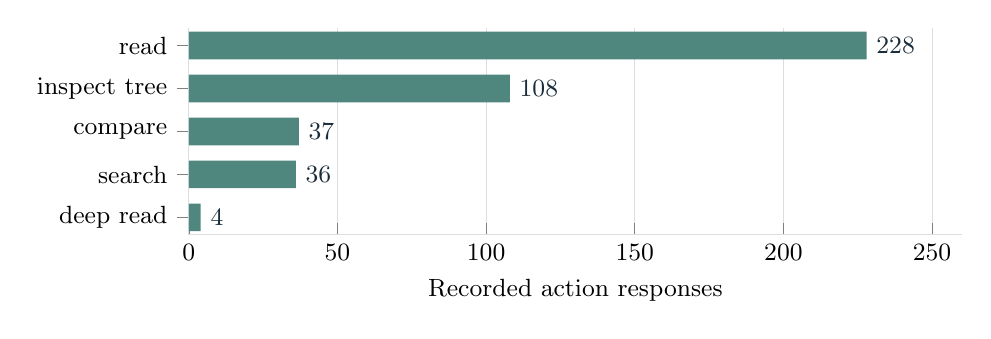
\begin{tikzpicture}
\begin{axis}[xbar,width=.94\linewidth,height=4.2cm,xmin=0,xmax=260,
 symbolic y coords={deep read,search,compare,inspect tree,read},ytick=data,
 tick label style={font=\small},xlabel={Recorded action responses},xlabel style={font=\small},
 axis x line*=bottom,axis y line*=left,axis line style={draw=linegray},
 xtick={0,50,100,150,200,250},xmajorgrids=true,grid style={linegray},
 nodes near coords,nodes near coords style={font=\small,text=ink},bar width=10pt]
\addplot[fill=accent!80,draw=none] coordinates {(4,deep read)(36,search)(37,compare)(108,inspect tree)(228,read)};
\end{axis}
\end{tikzpicture}
\captionof{figure}{Selected memory actions from the campaign. Frequent reads and tree inspections motivate testing whether more targeted retrieval can preserve discovery quality with less overhead.}
\end{center}

\newpage
\section{How this works}
At time $t$, the agent receives a bounded view of the current research tree, the task brief, and the available evidence references. It inspects the tree and selects a committed parent with a scored molecule as its comparison point. Parent selection determines the question's experimental lineage; it does not erase other branches or reset the campaign's best observed score.

\begin{center}
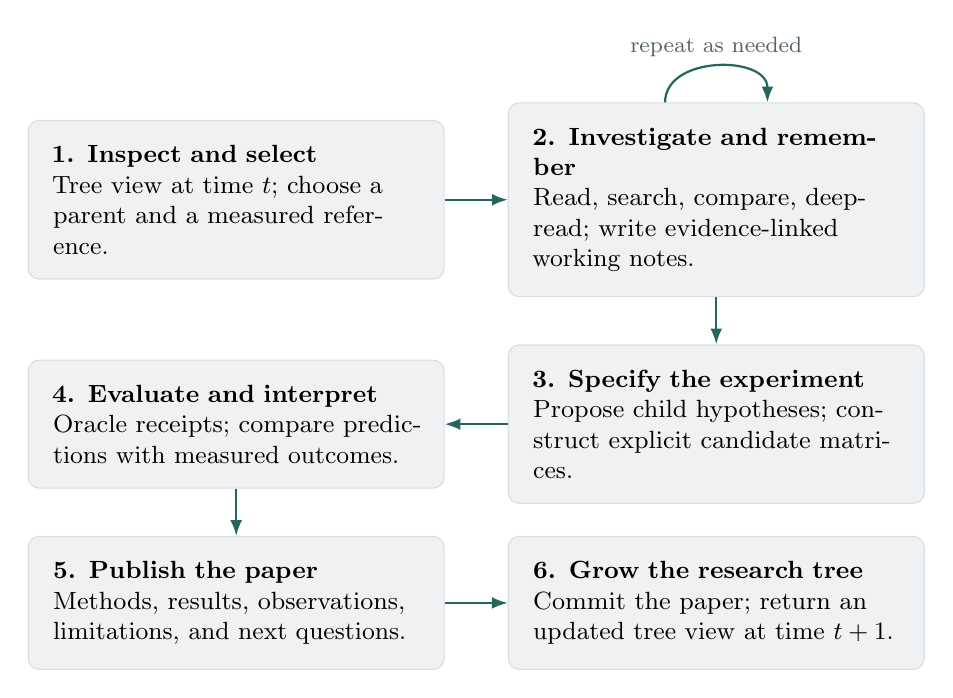
\begin{tikzpicture}
\node[flow] (a) {\textbf{1. Inspect and select}\\Tree view at time $t$; choose a parent and a measured reference.};
\node[flow,right=.8cm of a] (b) {\textbf{2. Investigate and remember}\\Read, search, compare, deep-read; write evidence-linked working notes.};
\node[flow,below=.6cm of b] (c) {\textbf{3. Specify the experiment}\\Propose child hypotheses; construct explicit candidate matrices.};
\node[flow,left=.8cm of c] (d) {\textbf{4. Evaluate and interpret}\\Oracle receipts; compare predictions with measured outcomes.};
\node[flow,below=.6cm of d] (e) {\textbf{5. Publish the paper}\\Methods, results, observations, limitations, and next questions.};
\node[flow,right=.8cm of e] (f) {\textbf{6. Grow the research tree}\\Commit the paper; return an updated tree view at time $t+1$.};
\draw[arrow](a)--(b);\draw[arrow](b)--(c);\draw[arrow](c)--(d);\draw[arrow](d)--(e);\draw[arrow](e)--(f);
\draw[arrow] ([xshift=-.65cm]b.north) .. controls +(0,.6cm) and +(0,.6cm) .. node[above,font=\footnotesize,text=muted]{repeat as needed} ([xshift=.65cm]b.north);
\end{tikzpicture}
\captionof{figure}{One research cycle. ReAct governs repeated decisions within the permitted phase; the experimental record persists across cycles.}
\end{center}

\textbf{Reasoning with working memory.} ReAct is the decision loop throughout the investigation. The agent can inspect a paper, observe a failed substitution, search for a related comparison, and write a note explaining how that result changes its next hypothesis. A dedicated reader can add a focused synthesis. These notes belong to the active workspace and can be cited or inherited by the subsequent hypothesis experiments.

\textbf{Turning a hypothesis into a test.} The agent states a claim, its rationale, a prediction, and an outcome that would challenge it. It then specifies a small matrix of starting structures and concrete interventions. Each cell contains the actual candidate molecule to be evaluated; the backend does not invent molecular edits. Freezing the matrix makes the intended experiment distinguishable from its subsequent interpretation.

\textbf{Closing the loop with evidence.} The backend validates and canonicalizes candidates, reuses cached scores for duplicates, and records new oracle evaluations. Invalid structures remain visible as construction failures. The observer compares the returned receipts with the prediction, then the reporter writes the full experiment paper. A Git-backed commit preserves the paper and verified matrix as a new tree node. Future decisions can retrieve its positive, negative, or inconclusive findings rather than relying on an ephemeral conversation.

\newpage
\section{An agent's trajectory}
The following trajectory reconstructs how the campaign moved from an unnamed starting structure to a much stronger observed candidate. Levels refer to experimental ancestry, not training steps. The narrative follows both improvements and the comparisons that changed the agent's understanding of which edits were worth pursuing.

\level{Level 0: establish the black-box problem}
The agent receives a complete task brief: propose valid molecules that improve an unknown scalar objective, using its tools and accumulated experimental memory. It is given one molecular structure with a measured score of \textbf{0.368} and no objective identity or scoring formula. At this point, it has no tested explanation for the low score. The initial record is therefore a baseline, rather than a completed hypothesis experiment, and the first task is to decide which structural changes could produce informative comparisons.

\level{Level 1: distinguish an attractive idea from a useful intervention}
The agent begins by testing two different directions. One hypothesis proposes aryl substitutions intended to alter electronic character or bulk; the two candidates both score \textbf{0.305}, below the starting point. A second hypothesis probes the terminal amine. Simple $N$-methylation also disappoints at \textbf{0.339}, but replacing the terminal group with a piperazinyl side chain raises the score to \textbf{0.857}. Together, these papers suggest that the side chain is a more promising research direction than the tested aryl edits. They do not establish that basicity or lipophilicity caused the gain: several properties changed together, leaving a question for the next level.

\level{Level 2: test competing explanations for the gain}
The agent now uses the successful parent as a basis for more discriminating experiments. Distal $N$-alkylation lowers the best score to \textbf{0.849}; halogen replacements reach \textbf{0.797}; morpholine and piperidine substitutions tie the reference at \textbf{0.857}. Ester and linker changes also fail to improve it. These comparisons narrow the useful search directions instead of merely generating more neighbors. The productive hypothesis concerns terminal-ring size: expansion to seven members gives \textbf{0.844}, while contraction to five gives \textbf{0.871}. The agent can now formulate a specific next test: does further ring contraction continue the measured improvement?

\begin{center}
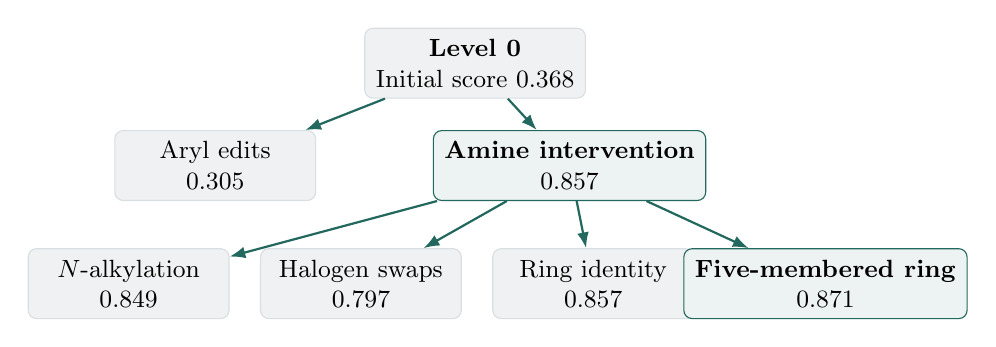
\begin{tikzpicture}[font=\small, every node/.style={align=center},
 n/.style={draw=linegray,fill=chipgray,rounded corners=3pt,minimum width=2.55cm,minimum height=.77cm,inner sep=4pt},
 w/.style={n,draw=accent,fill=accent!8},e/.style={arrow}]
\node[n] (r) at (0,0) {\textbf{Level 0}\\Initial score 0.368};
\node[n] (a) at (-3.3,-1.3) {Aryl edits\\0.305};
\node[w] (b) at (1.2,-1.3) {\textbf{Amine intervention}\\0.857};
\node[n] (c) at (-4.4,-2.8) {$N$-alkylation\\0.849};
\node[n] (d) at (-1.45,-2.8) {Halogen swaps\\0.797};
\node[n] (e) at (1.5,-2.8) {Ring identity\\0.857};
\node[w] (f) at (4.45,-2.8) {\textbf{Five-membered ring}\\0.871};
\draw[e](r)--(a);\draw[e](r)--(b);
\draw[e](b)--(c);\draw[e](b)--(d);\draw[e](b)--(e);\draw[e](b)--(f);
\end{tikzpicture}
\captionof{figure}{Selected early experiments. Green outlines identify improvements along the lineage continued below. Each child is an experiment; labels report its best candidate score.}
\end{center}

\newpage
{\large\sffamily\bfseries\color{ink}Agent trajectory, continued}\par
\level{Levels 3 and 4: turn a trend into better experiments}
At level 3, the agent extends the ring-size hypothesis while testing whether the improvement can instead be obtained through a core edit. A four-membered terminal ring reaches \textbf{0.889}, whereas removing or extending the core methyl lowers the score. A methyl-substituted five-membered ring also underperforms the four-membered candidate. The next experiment is therefore motivated by an accumulated trend, rather than a generic preference for smaller molecules. At level 4, the agent tests a three-membered diaza ring against an unchanged four-membered reference and reaches \textbf{0.905}, the best score observed in this campaign. A separate four-membered nitrogen-position isomer ties its parent, providing no evidence that nitrogen adjacency is a positive optimization lever.

\begin{center}
\begin{tabular}{@{}c@{\hspace{.6cm}}c@{}}
\includegraphics[width=.43\linewidth,height=3.5cm,keepaspectratio]{figs/l0.png} &
\includegraphics[width=.43\linewidth,height=3.5cm,keepaspectratio]{figs/l1.png}\\[-2pt]
{\small\textbf{Level 0} $\cdot$ 0.368} & {\small\textbf{Level 1} $\cdot$ 0.857}\\[6pt]
\includegraphics[width=.43\linewidth,height=3.5cm,keepaspectratio]{figs/l2.png} &
\includegraphics[width=.43\linewidth,height=3.5cm,keepaspectratio]{figs/best.png}\\[-2pt]
{\small\textbf{Level 2} $\cdot$ 0.871} & {\small\textbf{Level 4} $\cdot$ 0.905}
\end{tabular}
\captionof{figure}{Selected structures along the improving lineage: initial molecule, level-1 cyclic-amine candidate, level-2 five-membered ring, and level-4 three-membered ring. Scores rise from 0.368 to 0.857, 0.871, and 0.905; the intermediate level-3 result is 0.889.}
\end{center}

\level{Levels 5 and 6: revise the explanation and map the limits}
The later experiments improve the agent's account of what matters even when they do not improve the incumbent. Removing one or both nitrogens from the terminal three-membered ring preserves the \textbf{0.905} score, challenging the idea that the two-nitrogen pattern is essential. Ring enlargement, several linker edits, core $N$-alkylation, and further aryl changes fail to exceed that value. The accumulated evidence favors retaining a compact terminal ring and much of the existing scaffold, while leaving the hidden scoring mechanism unresolved. Some later experiments revisit cached comparisons, revealing a practical opportunity for better retrieval and parent selection. The outcome is a best-observed candidate and a record of tested alternatives, rather than a claim of a unique or global optimum.

\newpage
\section{Research agenda and expected contribution}
The next study should test whether explicit experiment papers improve discovery relative to simpler memory designs. Evaluate complete campaigns across independent runs and additional hidden objectives, with matched oracle and model-token budgets.

\subsection*{Evaluation design}
\begin{tabularx}{\linewidth}{@{}p{.29\linewidth}X@{}}
\toprule
\textbf{Comparison} & \textbf{Question it answers}\\
\midrule
Full hypothesis tree & How well does the complete retrieval, experimentation, and publication loop discover stronger candidates?\\[5pt]
Flat paper archive & Does explicit ancestry improve decisions beyond having the same searchable papers?\\[5pt]
Limited persistent memory & How much do retained experimental results and limitations contribute to later choices?\\[5pt]
Targeted retrieval policy & Can more selective reading reduce token cost and repeated experiments without reducing discovery quality?\\
\bottomrule
\end{tabularx}

\textbf{Primary outcomes.} Report best score against unique oracle evaluations, calls to prespecified score thresholds, variation across runs, and model-token cost. Count cached candidates separately from new evaluations.

\textbf{Learning quality.} Audit whether later hypotheses cite relevant results and discriminate among competing explanations. Track invalid constructions, redundant proposals, branch revisits, and papers that provide useful evidence without a score improvement. This tests whether accumulated memory improves the search strategy.

\subsection*{Two directions for improving the agent}
\textbf{Learn a more selective tool policy.} The action profile shows substantial reading and tree-inspection activity. Supervised fine-tuning or reinforcement learning could encourage targeted retrieval, useful note writing, and informative comparisons. The objective should balance discovery quality with model and oracle cost; a lower number of reads is valuable only if the agent retains the evidence needed for good experimental decisions.

\textbf{Improve search across the research tree.} Better parent selection could combine promising scores with unresolved scientific questions, evidence coverage, and the expected value of a comparison. Longer deliberation may be useful when several papers support incompatible explanations. Adaptive experiment allocation should be evaluated against the frozen-matrix prototype, with the same accounting for calls, duplicates, and construction failures.

\subsection*{Expected contribution}
The intended result is a reusable architecture coupling molecular search with persistent experimental memory. Success would show that accumulated evidence improves experiment selection and discovery efficiency, with every gain traceable to a candidate, an oracle receipt, and an evidence-grounded paper.

\vfill
{\footnotesize\color{muted}\textbf{Evidence basis.} Campaign-v2 ledger and committed experiment papers. The 83 unique scored molecules comprise initialization and 82 newly scored matrix cells; cached and invalid cells are excluded. Forty-eight experiment papers were completed. Proposed comparisons above are future work.}
\end{document}
